\chapter{Energieopslagsysteemkeuze}
\label{ch:energiekeuze}
In dit hoofdstuk worden de verschillende mogelijkheden voor een energieopslagsysteem bekeken. Eerst worden in paragraaf 3.1 de eisen aan het systeem toegelicht. Daarna worden in paragraaf 3.2 alle mogelijke energieopslagsystemen gecategoriseerd en wordt onderzocht of ze geschikt zijn voor dit project. Na de inventarisatie van deze systemen wordt in paragraaf 3.3 aan de hand van een model de keuze ingeperkt, waarna in paragraaf 3.4 de definitieve keuze wordt gemaakt door middel van een gewogen-criteria-analyse.

\section{Stroomschema energieopslagsysteemkeuze}
Op de volgende pagina staat een stroomschema, dit schema gaat langs verschillende eisen. Wanneer een systeem voldoet aan de eis stroomt hij door naar de volgende eis. Uiteindelijk worden de laatste resultaten aan de hand van prestatiecriteria beoordeeld en de optimale keuze geselecteerd. Al deze eisen worden verder in het hoofdstuk in detail besproken.
\begin{figure}[H]
    \centering
    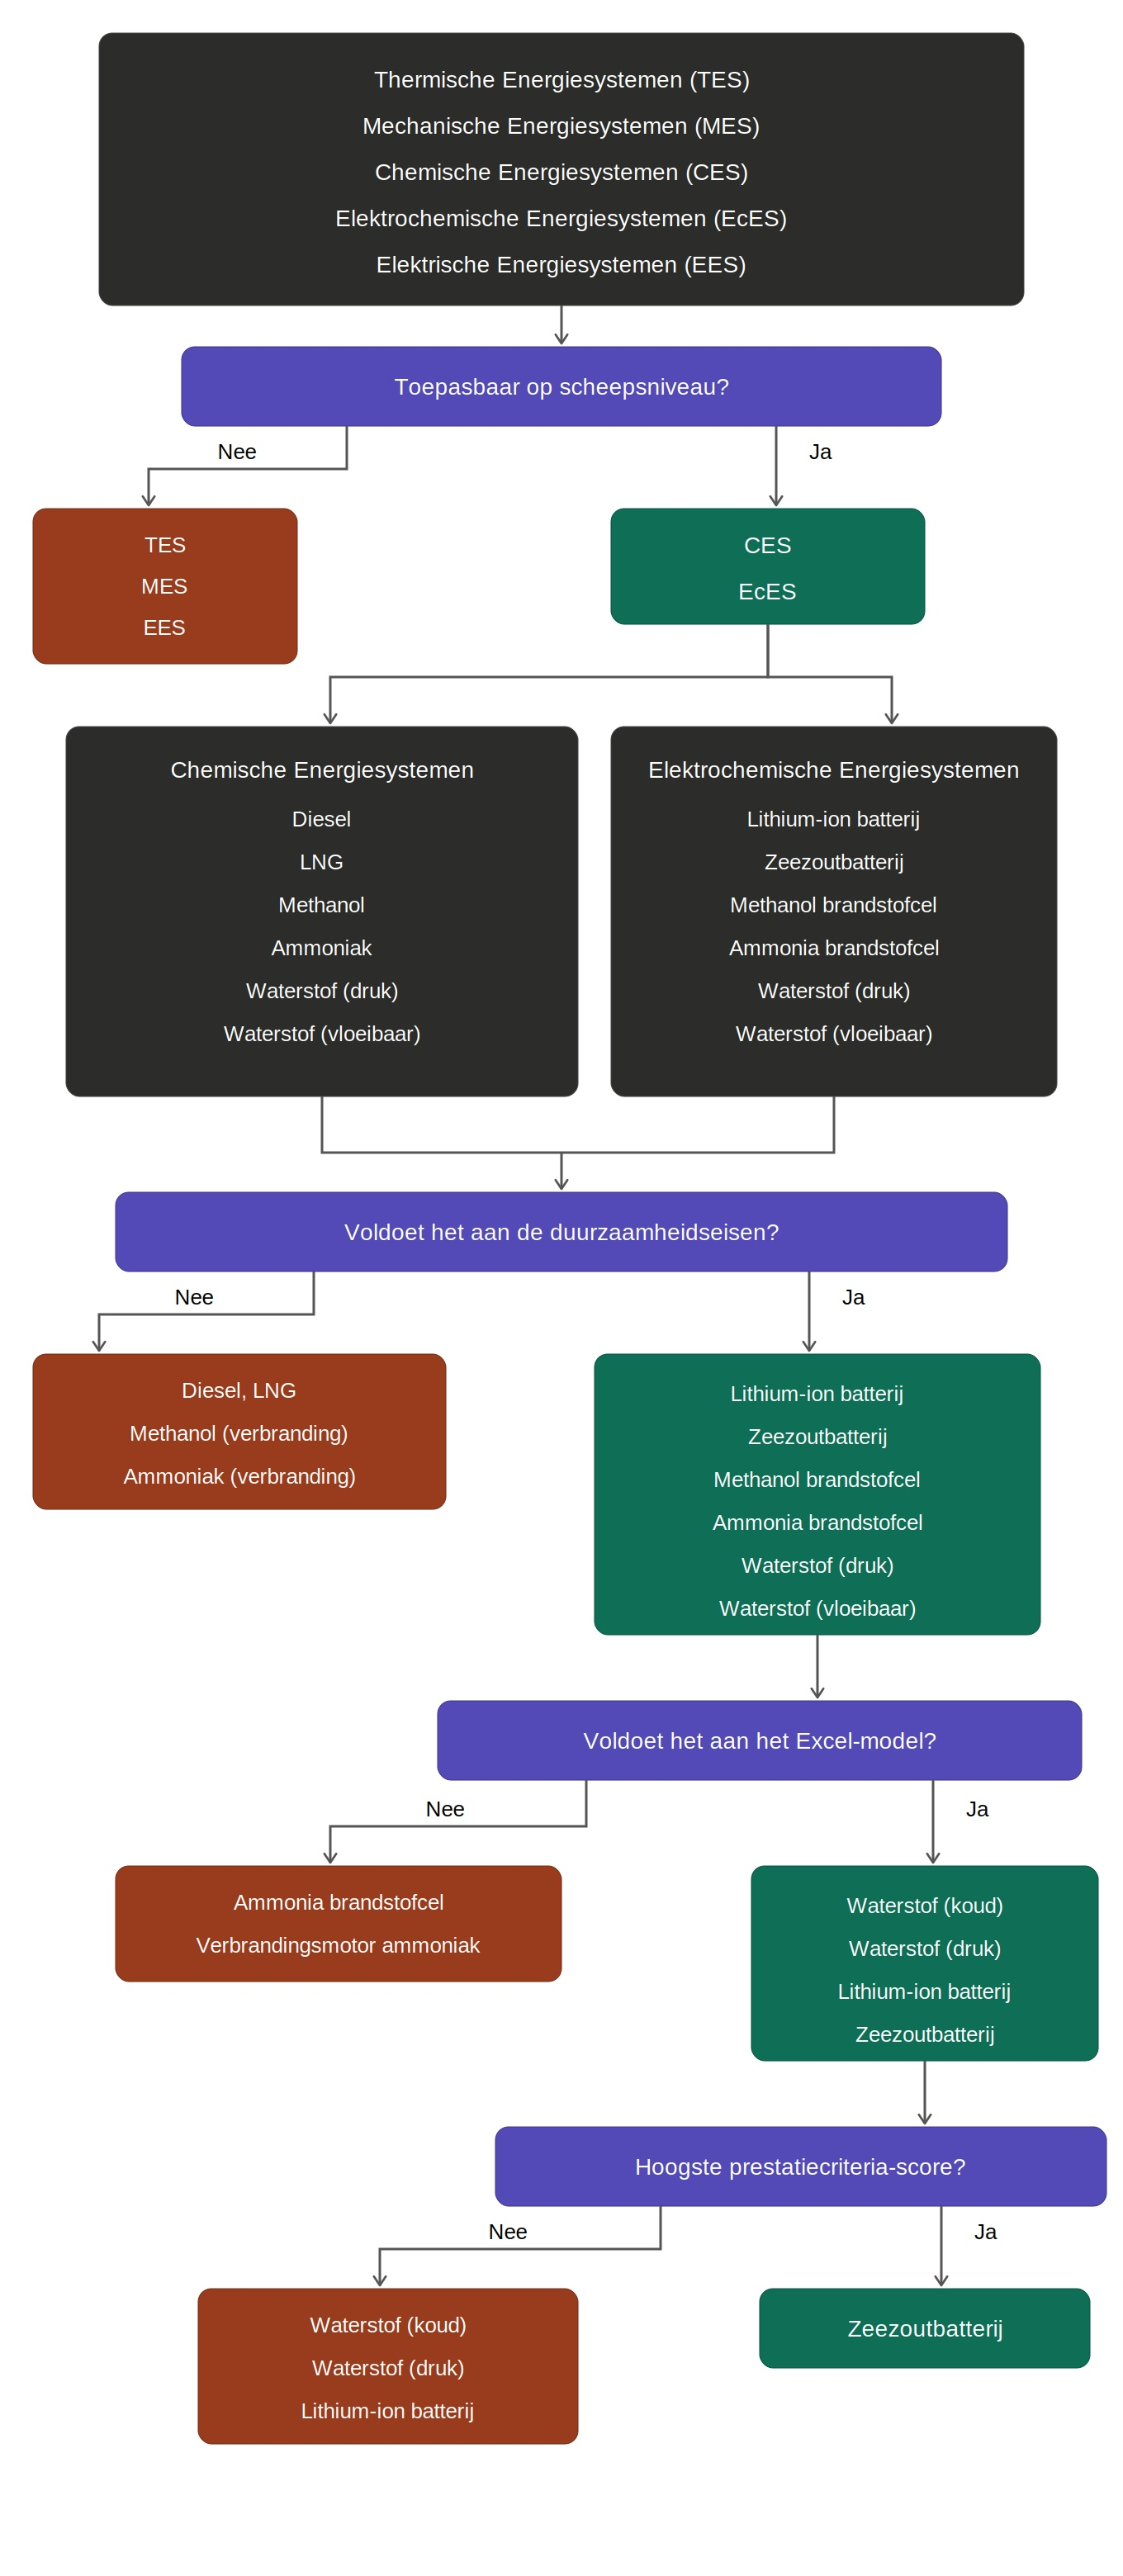
\includegraphics[width=0.65\linewidth]{Stroom.jpg}
    \caption{Stroomschema selectie opslagsysteem.}
    \label{stroomschema}
\end{figure}


\section{Algemene energieopslagsystemen}

Om in dit project een optimaal resultaat te behalen, is het van belang uit te zoeken welke mogelijkheden er zijn voor het opslaan van energie. Daarom is eerst gekeken naar alle categorieën energiesystemen. Gebruikmakend van de categorisering van energieopslagsystemen in J. Mitali et al \cite{mitali2022energy}, zijn een aantal categorieën geïdentificeerd. Om het onderzoek goed te beginnen, zal hiervan eerst bekeken worden of ze geschikt kunnen zijn voor het Jansje. Dit wordt in Tabel \ref{tab:vergelijking_energiesystemen} gedaan.

\begin{table}[h]
\centering
\caption{beschikbaarheid energiesystemen.}
\begin{tabular}{lcccccccc}
\toprule
Energiesysteem categorie & grootte & vermogen & energiedichtheid\\
\midrule
Thermmische energiesystemen (TES)   & x & x & \cmark\\
Mechanische energiesystemen (MES)   & x & \cmark & x\\
Chemische energiesystemen (CES)   & \cmark & \cmark & \cmark\\
Elektrochemische energiesystemen (EcES)  & \cmark & \cmark & \cmark\\
Elektrische energiesystemen (EES)   & x & \cmark & \cmark\\
Hybride energiesystemen (HES)   & x & x & x\\
\bottomrule
\end{tabular}
\label{tab:vergelijking_energiesystemen}
\end{table}

\noindent Zoals uit bovenstaande tabel te lezen is, zijn de categorieën Chemische-, Elektrochemische- en hybride energiesystemen geschikt voor dit project. Echter is er een beperkte tijd beschikbaar is voor dit project. daarom zullen de hybride systemen niet expliciet behandelt worden.

\subsection{Chemische energiesystemen (CES)}
Hieronder vallen systemen met fossiele energiedragers, zoals diesel, LNG, methanol, ammoniak en waterstof. Hoewel een aantal van deze energiedragers een CO$_2$-uitstoot heeft, kunnen deze brandstoffen verkregen worden zonder een netto uitstoot te creëren.

\subsection{Elektrochemische energiesystemen (EcES)}
Onder elektrochemische energiesystemen vallen batterijen. Dit is interessant voor dit project, omdat ze voldoende energie kunnen leveren en opnemen zonder de limieten voor beschikbaar volume en gewicht te overschrijden. Daarnaast zijn deze systemen relatief eenvoudig aan te sluiten op duurzame energiebronnen. Met walstroom zou een elektrochemisch energiesysteem bruikbare mogelijkheden kunnen bieden.

\section{Identificatie van mogelijke energieopslagsystemen}
In deze paragraaf worden voor de bovengenoemde categorieën specifieke energieopslagsystemen onderzocht. Als basis voor dit onderzoek is uitgegaan van een studie door een eerder studententeam aan de TU Delft. Zij hebben onderzocht hoe aan de hand van een model een keuze kan worden gemaakt voor een energieopslagsysteem van een willekeurig schip \cite{BEPmodelexcel}. Vanuit dit model zijn systemen overgenomen. Vervolgens zijn hier door literatuuronderzoek en overleg met de opdrachtgever en partners enkele systemen aan toegevoegd om aan te sluiten bij moderne technologie en een weloverwogen keuze te kunnen maken.

\subsection{Chemische energiesystemen}
Voor toepassing aan boord van Het Jansje is niet alleen de hoeveelheid energie
van belang, maar ook de manier waarop de brandstof wordt opgeslagen. De
opslagvorm bepaalt namelijk de benodigde tank, het volume, de massa, de
veiligheidseisen en de praktische toepasbaarheid aan boord. Daarom worden in
deze paragraaf verschillende chemische energiedragers vergeleken. We maken voor overzichtelijkheid ook verschil in verbranding en fuel cell.

\subsection*{Verbranding}

\subsubsection{\textbf{Diesel}}
Diesel is een fossiele brandstof die momenteel wordt gebruikt als energiebron voor de voortstuwing van het Jansje. Diesel is vloeibaar bij omgevingstemperatuur en kan eenvoudig worden opgeslagen. In een dieselmotor vindt verbranding plaats door compressieontsteking. Tijdens de verbranding komen echter grote hoeveelheden CO$_2$ en andere emissiegassen vrij, waardoor diesel geen duurzame energiebron is.

\subsubsection{\textbf{LNG}}
Liquefied Natural Gas (LNG) is aardgas dat vloeibaar wordt gemaakt door het af te koelen tot ongeveer −162 °C \cite{LiquefiedNaturalGasBook}. LNG kan worden toegepast in aangepaste verbrandingsmotoren met vonkontsteking. In vergelijking met diesel veroorzaakt LNG minder CO$_2$-uitstoot en minder andere emissies, maar het blijft een fossiele brandstof en is daarom geen volledig duurzame oplossing.

\subsubsection{\textbf{Methanol}}
Methanol (CH$_3$OH) is bij kamertemperatuur een vloeibare alcohol die kan worden toegepast als alternatieve brandstof in aangepaste verbrandingsmotoren. Bij verbranding komt minder CO$_2$ vrij dan bij diesel, maar methanol bevat koolstof, waardoor er nog steeds emissies ontstaan. Wanneer methanol wordt geproduceerd uit hernieuwbare energiebronnen (groene methanol), kan het wel als duurzame energiedrager worden beschouwd.

\subsubsection{\textbf{Ammoniak}}
Ammoniak (NH$_3$) is vloeibaar bij temperaturen onder −33 °C of een lichte overdruk \cite{EngineeringToolboxAmmonia}. Ammoniak bevat geen koolstof en veroorzaakt daarom geen directe CO$_2$-uitstoot bij verbranding. Wel kunnen er stikstofoxiden ontstaan tijdens het verbrandingsproces. Ammoniak kan worden toegepast in aangepaste verbrandingsmotoren of als energiedrager voor waterstofproductie en nog op diverse andere manieren.

\subsubsection{\textbf{Waterstof}}
Waterstof kan worden opgeslagen op twee manieren, of door middel van een combinatie hiervan. De eerste manier is opslag als vloeibare waterstof (−253 °C). Daarnaast kan waterstof worden opgeslagen als samengeperst gas onder hoge druk \cite{EngineeringToolboxHydrogen}. Als waterstof onder druk wordt opgelsagen kost het opslagproces 5-20\% van de energie die je uit waterstof kunt halen, afhankelijk van de grootte van de druk waarop je het brengt. Als waterstof afgekoeld moet worden tot het vloeibaar is kost het 30-40\% van de te gebruiken energie in de waterstof zelf, ook kost het energie om het gekoeld te houden \cite{doe2009hydrogencompression}. Vloeibaar waterstof is veel ingewikkelder om te gebruiken en kost dus ook veel meer energie. Aangezien er op het Jansje veel ruimte is en het om een 'klein' schip gaat wordt vloeibaar waterstof niet meegenomen.
Waterstof kan worden gebruikt in een verbrandingsmotor. De duurzaamheid van waterstof hangt sterk af van de productiewijze. In dit verslag wordt er uitgegaan van groene waterstof, dat is waterstof dat met duurzame elektriciteit is gemaakt. Bij de verbrandingsreactie ontstaat alleen H$_2$O, daarmee is het zo goed als emissievrij. Bij hoge temperaturen kan alsnog NO$_x$ ontstaan.



\subsection*{Fuel Cells}
\subsubsection{\textbf{Direct Methanol Fuel Cell}}
Dr. Ten werkt samen met het bedrijf SFC Energy en beval ons aan om de methanol fuel cell mee te nemen in het onderzoek. Een methanol fuel cell verbrandt geen methanol, maar maakt elektriciteit uit methanol en zuurstof door een elektrochemische reactie. Uit deze reactie ontstaan waterdamp, warmte en CO$_2$ \cite{SFCMethanolFuelCell}. De voordelen van dergelijke methanol fuel cell zijn dat de methanol makkelijk is op te slaan en te vervoeren, omdat het bij kamertemperatuur vloeibaar is. Een nadeel is dat het lokaal CO$_2$ uitstoot en dat het giftig is. Giftige vloeistoffen opslaan op een schip neemt risico's met zich mee \label{methanolgiftig}. Ook stoot het CO$_2$ uit, waardoor het niet volledig emissievrij is. Daarom is er besloten de methanol fuel cell niet verder mee te nemen in dit onderzoek.

\subsubsection{\textbf{Ammonia Fuel Cell}}
Een andere aanbeveling van Dr. Ten was om de GenCell FOX van GenCellEnergy te onderzoeken. Dat is een Ammonia Fuel Cell waarbij ammoniak niet als brandstof wordt gebruikt, maar als waterstofdrager. De ammoniak is opgeslagen in een tank en stroomt naar de 'cracker'. In de cracker wordt ammoniak (NH$_3$) opgesplitst in N en H$_3$ door een katalysator. De waterstof die daarbij vrij komt gaat naar de brandstofcel, waarin het zich bindt met zuurstof. Daarbij komt elektriciteit, water en stikstof vrij \cite{GenCellFOXVideo}. Omdat er geen CO$_2$ in ammoniak zit komt dat ook niet vrij en de stikstof die vrij komt is ongevaarlijk, omdat het al met grote hoeveelheden in de lucht zit. De voordelen van een Ammonia Fuel Cell zijn dat de reactieproducten emissievrij en ongevaarlijk zijn en ammoniak veel makkelijker is op te slaan dan alleen waterstof. Een nadeel is dat ammoniak giftig is en bij een kleine lekkage al gevaarlijk kan zijn \cite{NIPVAmmoniakincidenten} \label{Ammoniakgiftig}. Ook kan ammoniak vrijkomen bij onvolledige omzetting. Op een klein schip als Jansje is de vluchtruimte beperkt en zou een incident met ammoniak tot ernstige veiligheidsrisico's kunnen leiden. Daarom wordt ammoniak niet verder meegenomen in dit onderzoek.

\subsubsection{\textbf{Hydrogen Fuel Cell}}
Een Hydrogen Fuel Cell is een brandstofcel die waterstof (H$_2$) omzet in elektriciteit, warmte en H$_2$O. Waterstof komt de brandstofcel binnen en wordt door een katalysator gesplitst, waarbij elektronen vrijkomen. Ook wordt zuurstof uit de lucht toegevoegd om deze reactie mogelijk te maken. De voordelen zijn dat het emissievrij is, ongevaarlijk is en een hoge energiedichtheid heeft. Nadelen zijn dat de opslag van waterstof lastig is, omdat het bij een normale temperatuur en druk een hele lage dichtheid heeft. Om waterstof te kunnen gebruiken moet het daarom sterk gecomprimeerd opgeslagen worden. Dat kan gedaan worden door het op een hele hoge druk te brengen (300-700 bar) of extreem te koelen tot -253 c°C zodat het vloeibaar wordt en een veel hogere dichtheid krijgt \cite{EngineeringToolboxHydrogen}. Dit brengt extra risico's en veiligheidseisen met zich mee, waar rekening mee moet worden gehouden. Bij waterstof verbranding is uitgelegd waarom vloeibare waterstof niet meegenomen wordt.

\subsection{Elektrochemische energiesystemen}
In deze paragraaf zal worden gekeken naar de verschillende Elektrochemische systemen die er op de markt zijn en welke daarvan de beste optie zouden kunnen zijn voor dit project.


\subsection*{Lithium-ion batterijen}
Er zijn verschillende batterijen op de markt. Om de batterij te vinden die het meest geschikt is voor dit project, is gekeken naar een selectie die het meest gangbaar is voor de voortstuwing van schepen \cite{Szewczyk2023}:
\begin{itemize}
    \item Lithium-ijzer fosfaatbatterij (LFP)
    \item Lithium-nickel mangaankobaltoxide batterij (NMC)
    \item Nickel kobalt aluminiumoxide batterij (NCA)
    \item Grafiet/lithium-nickel mangaankobaltoxide batterij (G-NMC)
    \item Lithium mangaanoxide batterij (LMO)
    \item lithium titaanoxide batterij (LTO)
    \item Lithium kobaltoxide  batterij (LCO)
\end{itemize}

\noindent Voor deze batterijen zijn de volgende prestatiecriteria opgesteld:

\begin{itemize}
    \item \textbf{Veiligheid} Dit is afhankelijk van de aanwezigheid van giftige stoffen, en hoe groot de kans is op \textit{thermal runaway.}
    \item \textbf{Kosten} Hierbij wordt gekeken hoeveel een batterij kost ten opzichte van de alternatieven.
    \item \textbf{Levensduur} Dit is hoeveel laad- en ontlaadcyclussen de batterij mee kan gaan zonder zijn functie te verliezen.
    \item \textbf{Energiedichtheid} Onder energiedichtheid wordt verstaan de hoeveelheig energie (Wh) per gewicht (kg) in de batterij opgeslagen kan worden.
\end{itemize}



\noindent Daaruit volgt een criteriatabel. Door alle projectleden een stem te hebben gegeven in het bepalen van de wegingen, zijn de wegingen zo objectief mogelijk opgesteld.


\begin{table}[h]
\centering
\caption{prestatiecriteria tabel  van lithium-ion batterijen \cite{Szewczyk2023}}
\begin{tabular}{lcccccccc}
\toprule
Criteria & Weging (\%) & NMC & LFP & LTO & LCO & LMO & NCA & G-NMC \\
\midrule
Veiligheid          & 30 & 2 & 3 & 3 & 1 & 2 & 2 & 2\\
Kosten              & 20 & 2 & 2 & 1 & 2 & 3 & 3 & 2\\
Levensduur          & 20 & 1 & 2 & 3 & 1 & 1 & 1 & 3\\
Energiedichtheid    & 20 & 2 & 2 & 1 & 2 & 2 & 3 & 2\\
Totaal              & 100 & 1.8 & 2.3 & 2.0 & 1.5 & 1.8 & 2.0 & 2.2\\
\bottomrule
\end{tabular}
\label{tab:vergelijking_batterijen}
\end{table}

\noindent Hieruit blijkt dat LFP de meest geschikte batterij is voor dit project. Deze zal in het vervolgonderzoek worden meegenomen.

\subsubsection{\textbf{Zeezoutbatterij}}

Fieldlab Maassluis heeft een samenwerking met het bedrijf Dr Ten. Dr Ten is een innovatief bedrijf dat zich onder andere specialiseert in het ontwerpen van een zeezoutbatterij \cite{drten_zeezout_batterij2}. Om de volgende informatie te verkrijgen hebben meerdere online meetings plaatsgevonden met Marnix ten Kortenaar (oprichter en directeur van Dr Ten) en Gerrit (proces- en marketdeveloper). \\

\noindent De generatie 4.0 zeezoutbatterij werkt als volgt: in een cilinder bevindt zich een vloeibaar elektrolyt, onder andere bestaande uit een mengsel van zout water \cite{kouwenberg2023}. Verder is er een kathode en anode aanwezig van grafiet waar zink zich tijdens het laden aan vasthecht. Tijdens het ontladen, lossen deze zink-ionen weer op in het water, waarbij elektronen en energie vrijkomen. Deze batterijen zijn op dit moment enkel verkrijgbaar als demo model, de cellen worden met de hand gemaakt en daardoor zijn de kosten ook relatief hoog. Dr Ten is echter bezig met het automatiseren van het productieproces waardoor de prijzen kunnen concurreren met de prijs van lithium batterijen en naar verwachting zelfs lager worden. De eerste automatiseringsstappen zullen aankomende zomer ondernomen worden waarmee de productietijd viermaal sneller wordt. Tot op heden wordt de batterij vooral gebruikt voor statische toepassingen, hierom is een onzekerheid in hoeverre de batterij naar behoren functioneert in een maritieme toepassing. Onderzoek naar of dit complicaties zal opleveren is dan ook een vereiste.

\noindent Er zijn een aantal voordelen bij deze batterij ten opzichte van eerder genoemde batterijen. Allereerst is de kostprijs van de batterij, aldus Marnix ten Kortenaar, in de toekomst vele malen lager dan elke andere batterij. Verder is de batterij gebouwd met mineralen, koolstof soorten en zouten, dit zijn geen toxische materialen waardoor de veiligheid vele malen groter is dan bij andere batterijen \cite{DrTen1}. Daarnaast kan de zeezoutbatterij tijdens het gebruik volledig worden ontladen, wat bij de meeste andere batterijen de levensduur zeer significant verminderd \cite{DrTen1}. Ook is de degradatie na meer dan 50.000 cycli minimaal \cite{JIPBatteryMaassluis} \label{zeezout50000}. Een nadeel is echter het beperkte ontlaadvermogen; 1.46 W ontlaadvermogen ten opzichte van 3.3 W laadvermogen \cite{JIPBatteryMaassluis}. Dit kan risico's met zich meebrengen tijdens het varen, aangezien een kortstondige piek in vermogen nodig kan zijn om obstakels te ontwijken of aan te meren. \\

\noindent Om dit probleem op te lossen heeft Dr. Ten zelf een batterij gemaakt waarbij een zeezoutbatterij wordt gecombineerd met lithium, de zogeheten generatie  6.0. Deze batterij is echter in de laatste testfase waardoor hij niet beschikbaar is voor de markt, de verwachting is dat de batterij door de combinatie met lithium een aanzienlijk hoger ontlaadvermogen heeft waardoor dit probleem opgelost is.

\section{Duurzaamheidseisen}
Om het juiste energieopslagsysteem te kunnen selecteren, moet eerst worden gedefinieerd wat in dit project onder duurzame energie wordt verstaan. Volgens het NEA (Nederlandse Emissieatoriteit) \cite{NEAHernieuwbareEnergie} walstroom als groen beschouwd. Deze beschouwing is technisch gezien niet helemaal correct, maar zal gedurende dit project wel als de offciële maatstaf worden gebruikt \label{walstroomgroen}. Aan de hand van deze eisen zijn de volgende prestastiecriteria opgesteld:

\begin{itemize}
    \item Well-to-tank (WTT), hierbij wordt onderzocht hoeveel uitstoot er plaatsvindt tijdens het produceren van het energieopslagsysteem. Er wordt gekeken naar materiaalwinning en productieprocessen waarbij een score van 5 betekent dat alle materialen ruim aanwezig zijn, herwinbaar zijn en winning ervan lage impact heeft op het milieu.
    \itemTank-to-wake (TTW), hierbij wordt gekeken naar de emissies die plaatsvinden bij het aandrijven van het schip. Een score van 5 betekent dat er geen uitstoot plaatsvindt terwijl een score van 1 juist heel veel uitstoot toont.
    \item Circulariteit (circ.), bij dit criteria wordt onderzocht in hoeverre de energiebron uitputbaar is. Een score van 5 wordt gegeven als de energiebron onuitputbaar is, terwijl een score van 1 wordt gegeven als de energiebron eindig is.
    \item Milieurisico bij calamiteiten (falen) (Calam.), sommige energieopslagsystemen resulteren bij falen in uitstoot van zeer milieubelastende uitstoot. Deze krijgen dan ook een score van 1 terwijl zeer weinig uitstoot bij falen een score van 5 krijgt.
\end{itemize}

\noindent Elk projectlid heeft gestemd op welk criteria het belangrijkst bevonden wordt, aan de hand van deze stemmen \ref{naar google forms of citen ofz ff kijken hoe we dat flippen} zijn vervolgens de wegingen bepaald (afgerond op hele procenten). Wegens het feit dat voor bepaalde criteria zoals circulariteit en calamiteitenrisico geen empirische waarden te vinden zijn, zullen de verschillende systemen op basis van verschillende bronnen worden vergeleken en zal aan de hand daarvan een score worden bepaald.

\begin{table}[h]
\centering
\caption{Vergelijking van chemische energiedragers voor toepassing aan boord van Het Jansje}
\label{tab:chemische_energiedragers}
\renewcommand{\arraystretch}{1.3}
\footnotesize
\begin{tabular}{lcccc>{\centering\arraybackslash}p{1.6cm}}
\hline
\textbf{Energiedrager} &
\textbf{TtW emissies} &
\textbf{WtT emissies} &
\textbf{Circulariteit} &
\textbf{Calamiteiten-risico} &
\textbf{Totaal-score} \\
& \scriptsize(kg CO\textsubscript{2}/kWh) & \scriptsize(kg CO\textsubscript{2}/kWh) & & & \\
\hline
Diesel
  & 0.264 \cite{CO2Emissiefactoren2026}
  & 0.081 \cite{CO2Emissiefactoren2026}
  & 1 \cite{EIADieselExplained2024}
  & 4 \cite{PoisonControlGasolineDiesel}
  & D \\
LNG
  & 0.216 \cite{CO2Emissiefactoren2026}
  & 0.052 \cite{CO2Emissiefactoren2026}
  & 1 \cite{GHDEnergyLNG}
  & 2 \cite{CLNGSafety}
  & L \\
Methanol verbranding
  & 0
  & 0.005 \cite{CO2Emissiefactoren2026}
  & 3 \cite{KlineMethanol2024}
  & 3 [\ref{methanolgiftig}]
  & MV \\
Ammoniak verbranding
  & 0 \cite{IEAAMFAmmoniaEmissions}
  & 0 \cite{IEAAMFAmmoniaEmissions}
  & 4 \cite{IEAAMFAmmoniaEmissions}
  & 1 [\ref{Ammoniakgiftig}]
  & Av \\
Waterstof verbranding
  & 0 \cite{CO2Emissiefactoren2026}
  & 0.033
  & 4 \cite{DOEHydrogenStorage}
  & 2 \cite{UCSSafetyHydrogen}
  & WV \\
Methanol brandstofcel
  & 0 \cite{CO2Emissiefactoren2026}
  & 0.059\textsuperscript{a} \cite{Elsevier}
  & 3 \cite{KlineMethanol2024}
  & 3 [\ref{methanolgiftig}]
  & Mb \\
Ammoniak brandstofcel
  & 0 \cite{CO2Emissiefactoren2026}
  & 0.005\textsuperscript{a} \cite{Elsevier}
  & 3 \cite{IEAAMFAmmoniaEmissions}
  & 1 [\ref{Ammoniakgiftig}]
  & Ab \\
Waterstof brandstofcel (onder druk)
  & 0 \cite{CO2Emissiefactoren2026}
  & 0.038\textsuperscript{a} \cite{IEAAMFAmmoniaEmissions}
  & 4 \cite{DOEHydrogenStorage}
  & 2 \cite{UCSSafetyHydrogen}
  & Wb \\
LFP batterij
  & 0 \cite{GenCellFOXProduct}
  & 0.019 \textsuperscript{b} \cite{GjetaLCA2024}
  & 3 \cite{Bazzanini2024}
  & 3 \cite{DTGPowerLFPFire}
  & LFP \\
Zeezoutbatterij
  & 0 (\ref{walstroomgroen})
  & $\approx$0\textsuperscript{c} \cite{GjetaLCA2024}
  & 5 \cite{drten_zeezout_batterij2}
  & 0 \cite{drten_zeezout_batterij2}
  & Zeezout \\
\hline
\end{tabular}

\vspace{0.2cm}
\footnotesize
\begin{flushleft}
\textsuperscript{a} Inclusief +0.005 kg CO\textsubscript{2}/kWh voor brandstofcelproductie \cite{Elsevier}.\\
\textsuperscript{b} Totale impact berekend uit gemiddelde waarden voor materiaalwinning, productie en recycling, gewogen met levenscycli, efficiëntie en ontladingsdiepte $$ \text{WTT (Productie-deel)} = \frac{70\text{ kg}}{5.000 \times 0.8 \times 0.9} \approx {0.019\text{ kg CO}_2\text{/kWh}} $$ \cite{GjetaLCA2024}.\\
\textsuperscript{c} Productiedeel wordt gelijkwaardig door $\sim$50.000 laadcycli \ref{zeezout50000} verwaarloosbaar en gesteld op 0 kg CO\textsubscript{2}/kWh.
\end{flushleft}
\end{table}



\begin{table}[h]
\centering
\caption{Vergelijking van energiedragers op basis van scores (1-5)}
\label{tab:scores_energiedragers}
\renewcommand{\arraystretch}{1.2}
\begin{tabular}{lccccc}
\hline
\textbf{Energiedrager} & \textbf{TTW} & \textbf{WTT} & \textbf{Circ.} & \textbf{Calam.} & \textbf{Totaal} \\
\hline
\textbf{Weging (\%)} & \textit{32\%} & \textit{30\%} & \textit{23\%} & \textit{15\%} & \textit{100\%} \\
\hline
Diesel & 1 & 1 & 1 & 4 & 1.45 \\
LNG & 2 & 2 & 1 & 2 & 1.77 \\
Methanol verbranding & 5 & 5 & 3 & 3 & 4.24 \\
Ammoniak verbranding & 5 & 5 & 4 & 1 & 4.17 \\
Waterstof verbranding & 5 & 3 & 4 & 2 & 3.72 \\
Methanol brandstofcel & 5 & 2 & 3 & 3 & 3.34 \\
Ammoniak brandstofcel & 5 & 5 & 4 & 1 & 4.17 \\
Waterstof brandstofcel & 5 & 3 & 4 & 2 & 3.72 \\
LFP batterij & 5 & 4 & 3 & 3 & 3.94 \\
Zeezoutbatterij & \textbf{5} & \textbf{5} & \textbf{5} & \textbf{5} & \textbf{5.00} \\
\hline
\end{tabular}
\end{table}


\noindent Aangezien er nu gebruik wordt gemaakt van diesel, en dit verduurzaamd dient te worden valt deze keuze af. LNG scoort met een minimale hoeveelheid hoger dan diesel en zal dus niet als verduurzaming worden gezien gedurende dit project. Alle overige opties zullen verder worden meegenomen in het onderzoek.

\section{Modelresultaten}

\noindent In deze paragraaf wordt getoond hoe het model van het eerder genoemde studententeam \cite{BEPmodelexcel} is aangevuld met de nieuwe energiesystemen, geactualiseerd met waarden van het huidige marktaanbod, en wat de uiteindelijke resultaten zijn. De toegevoegde energiesystemen zijn de zeezoutbatterij ($4^e$ generatie) en de fuelcell op ammoniakbasis.

\subsection{Invoer}
\begin{figure}[H]
    \centering
    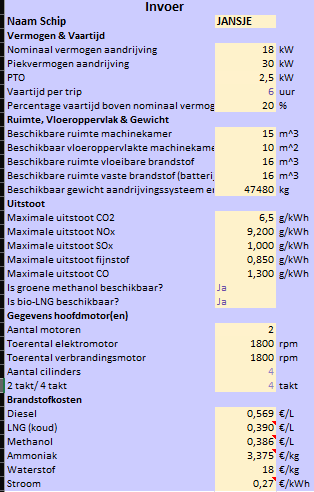
\includegraphics[width=0.5\linewidth]{Invoer-Uitvoer.png}
    \caption{Invoer van het excel model}
    \label{fig:invoer_model}
\end{figure}
Om dit model te kunnen gebruiken, zijn een aantal aannames en schattingen gemaakt.
Voor het vermogen en de vaartijd zijn grote delen al bepaald bij hoofdstuk 4 (?).\\
Ook zijn voor de ruimte, het vloeroppervlak en het gewicht  een schatting gemaakt op basis van de scheepsdimensies.\\
Daarnaast wordt van de maximale uitstoot  verwacht dat het systeem minimaal voldoet aan de europese richtlijnen \cite{Europeanstandards}.\\
Tevens zijn de gegevens van de hoofdmotoren  bepaald door een interview met de eigenaar.\\
Als laatste is er voor de brandstofkosten simpelweg gekeken naar diverse bronnen over de huidige prijzen om zo te komen tot een onderbouwde prijs \cite{Brandstofprijs} \cite{LNGprijs} \cite{Waterstofguide}.



\subsection{Data}
\subsection{Uitvoer}
\begin{figure}[H]
    \centering
    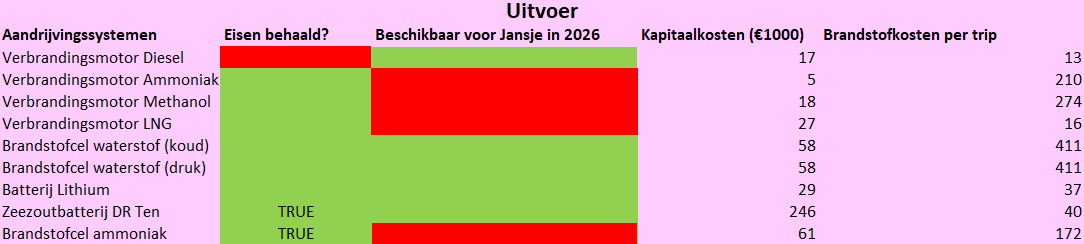
\includegraphics[width=0.7
    \linewidth]{Hoofdstukken/uitvoer.png}
    \caption{Caption}
    \label{fig:uitvoer_model}
\end{figure}



\section{Systeemconfiguratie en Randvoorwaarden}
Om de keuze voor het energieopslagsysteem te maken, wordt gebruik gemaakt van een gewogen criteria analysetabel. Om deze tabel correct in te vullen, is het van belang om de systeemconfiguraties te bepalen voor de drie overgebleven energieopslagsystemen. De gekozen systemen zijn: de lithiumbatterij LFP 24V IP van MG Energy \cite{mg_lfp_datasheets_page_2026}, omdat deze geschikt is voor ruige maritieme doeleinden. Een zeezoutbatterij van Dr. Ten (24 V, 20 Ah) \cite{DrTenInfo2025} en een druktank met brandstofcel voor waterstof van \cite{powercell_s2_fuel_cell_stack} \cite{holthausen_telefoon_2026}.\\

\noindent In tabel 5.7 worden van elk van deze systemen de specificaties getoond:

\begin{table}[h]
\centering
\caption{Informatie Potentiele Energieopslagmethoden}
\resizebox{\textwidth}{!}{
\begin{tabular}{lccccc}
\toprule
Criterium & LFP \cite{mg_price_list_2026} \cite{mg_lfp_datasheets_page_2026} \cite{independer2026stroomprijs} \cite{redondoiglesias2022efficiency} & Zeezoutbatterij (gen 4.0) \cite{drten_zeezout_batterij2} \cite{JIPBatteryMaassluis} \cite{independer2026stroomprijs} \cite{DrTenInfo2025} & Waterstof brandstofcel
\cite{powercell_s2_fuel_cell_stack}
& Waterstof Tank (Druk) \cite{holthausen_telefoon_2026}
\cite{h2live_2026}
\cite{nationalacademies_hydrogen_energy_content}\\
\midrule
Capaciteit (kWh) & 5.8 &  0.48 & n.v.t. & 234\\
Vermogen (kW)  & 5.89 & 0.187 & 26 & n.v.t\\
Aankoopprijs (€) &  2.468 & 2.104 & 52.000 \cite{vertrouwelijk_telefoongesprek_fuelcell_2026} & 10.500\\
Kosten volledigde laadcyclus (€)& 1,40 & 0,12 & n.v.t. & 142 \\
Massa (kg) & 40 & 18.7 & 28.5 & 154.5 Kg (tank) + 7.1 Kg (waterstof)\\
Dimensies (L x B X H (m)) & 0.531 x  0.206 x 0.295& 0.60 x 0.39 x 0.23 & 0.155 x 0.490 x 0.358 & 3.0 x 0.42 x 0.42 \\
Efficiëntie (\%) & 92 & 97 & 57 & n.v.t\\
\bottomrule
\end{tabular}
}
\label{tab:prestatievergelijking_uitgebreid}
\end{table}


\noindent Nu de algemene eigenschappen van de energieopslagsystemen compleet in beeld zijn kunnen deze worden omgevormd zodat ze voldoen aan het benodigd vermogen van 22.5 kW \ref{} en de benodigde capaciteit van 108.15 kWh \ref{}. 0m te voldoen aan deze eisen wordt in deze tabel gerekend met:
\begin{itemize}
    \item 26 LFP batterijen
    \item 233 Zeezoutbatterijen
    \item 1 waterstof tank (?L) en 1 waterstof brandstofcel
\end{itemize}

\begin{table}[h]
\centering
\caption{Informatie specifieke energieopslag}
\resizebox{\textwidth}{!}{
\begin{tabular}{lccccc}
\toprule
Criterium & LFP & Zeezoutbatterij (gen 4.0) & Waterstof brandstofcel + Tank \\
\midrule
Benodigde capaciteit (kWh) & 146.95 & 111.49 & 189.74\\
Aankoopprijs (€) &  64.168 & 490.232 & 52.000 + 10.500\\
Kosten per effectieve kWh (€/ kWh)& 0,261 & 0,247 & 1,05\\
Massa (kg) & 1040 & 4357,1 & 28.5 + 154 Kg (tank) + 7.1 Kg (waterstof))\\
Volume (m^3) & 0.05382 & 12.54 & 0.5564 \\
Efficiëntie (\%) & 92 & 97 & 57 \\
Innovativiteit (\%) & 2.6 & 4.6 & 4.0\\
Duurzaamheid & 3.94 & 5.00 & 3.72 \\
Veiligheid & 3.4 & 4.3 & 2.0 \\
Levensduur (jaren) & 87.5 & 1250 & 125 \\

\bottomrule
\end{tabular}}
\label{tab:specifieke_energieopslag}
\end{table}

Deze nog naar de bijlage

\begin{table}[h]
\centering
\caption{Berekening Informatie specifieke energieopslag}
\resizebox{\textwidth}{!}{
\begin{tabular}{lccccc}
\toprule
Criterium & LFP & Zeezoutbatterij (gen 4.0) & Waterstof brandstofcel + Tank \\
\midrule
Effectieve Capaciteit (kWh) & 108,15 & 108,15 & 7.1 \times 33.3 \times 0.57 \approx 134.77\\
Aankoopprijs (€)&  2.468 \times 26 = 64.168 & 2.104 \times 233 = 490.232 & 52.000 + 10.500\\
Kosten per effectieve kWh (€/ kWh)& $ \frac{1}{0.92}$ \approx 1.087 \times 0.24 \approx 0.261 & $\frac{1}{0.97}$ \approx 1.03 \times 0.24 \approx 0.247 & 33.3 \times 0.57 \approx 18.98 --> $\frac{20}{18.98}$ \approx 1.05 \\
Massa (kg) & 40 \times 26 = 1040 & 18.7 \times 233 = 4357,1 & 28.5 + 154 Kg (tank) + 7.1 Kg (waterstof))\\
Efficiëntie (\%) & 92 & 97 & 57 \\
Innovativiteit (\%) & 2.6 & 4.6 & 4.0\\
Duurzaamheid  & 3.94 & 5.00 & 3.72 \\
Veiligheid & 3.4 & 4.3 & 2.0 \\
Levensduur (jaren) & 87.5 & 1250 & 125 \\

\bottomrule
\end{tabular}}
\label{tab:berekening_energieopslag}
\end{table}


Nu in beeld is gebracht wat er voor elk systeem benodigd is kan er worden onderzocht of de systemen in deze configuratie aan de volgende randvoorwaarden doen:

\begin{itemize}
    \item Het minimaal benodigd vermogen is 22.5 kW.
    \item Het maximaal beschikbaar toe te voegen gewicht bedraagt 36.180 kg \ref{berekeningvan Aymen}, een hoger gewicht zou namelijk resulteren in zinken van het schip.
    \item Het maximaal beschikbaar volume in de machinekamer en het laadruim is 12 $m^3$ \cite{vanbaalen2026interview}/ berekening van Milan.
    \item Om te voldoen aan de eis van scheepseigenaar Wim van Baalen is het van belang dat de minimale levensduur die het systeem moet kunnen doorgaan voordat het rendement dusdanig afneemt dat het systeem vervangen moet worden 10 jaar is \cite{vanbaalen2026interview}.
\end{itemize}

\begin{table}[h]
\centering
\caption{Tabel van energieopslagmethoden specifiek voor Jansje}
\resizebox{\textwidth}{!}{
\begin{tabular}{lcccccc}
\toprule
Randvoorwaarde & LFP & Zeezoutbatterij & Waterstof (druk)  \\
\midrule
Massa (Kg) & \cmark & \cmark   & \cmark&\\
Ontlaadvermogen (W) & \cmark & \cmark &  \cmark \\
Volume (m$^3$) & \cmark &  \xmark  & \cmark & \\
Levensduur (jaren)& \cmark & \cmark & \cmark & \\
\bottomrule
\end{tabular}
}
\label{tab:randvoorwaarden_check}
\end{table}

\subsection*{Conclusie}
\noindent Uit bovenstaande tabel valt af te lezen dat zowel de LFP-batterij als de waterstof brandstofcel voldoen aan alle randvoorwaarden. Dit betekent dan ook dat beide direct op het schip geïmplementeerd zouden kunnen worden. Voor de zeezoutbatterij geldt echter dat er niet wordt voldaan aan de randvoorwaarde van het volume, het systeem is te groot en past daardoor niet in het schip. Mocht de zeezoutbatterij als beste systeem uit het onderzoek komen zal dan ook onderzocht moeten worden of dit probleem op te lossen is, zodat het alsnog voldoet aan alle gestelde randvoorwaarden.

\section{Gewogen criteria analyse}


\noindent Nu uitsluitend de energieopslagsystemen zijn overgebleven die beschikbaar en toepasbaar zijn voor transportschip het Jansje, is het van belang om te onderzoeken welke het beste geschikt is. Dit wordt gedaan aan de hand van een gewogen-criteria analyse, waarin prestatiecriteria zijn opgesteld en scores zijn toegekend op basis van verschillende bronnen. Na het invullen van deze tabel wordt duidelijk welk energieopslagsysteem het best past bij dit project. De prestatiecriteria zijn als volgt:

\begin{itemize}
    \item \textbf{Duurzaamheid}: Met duurzaamheid wordt onderzocht hoe het systeem scoort op basis van de duurzaamheidseisen \ref{}, het meest duurzame systeem ontvangt de hoogste score.
    \item \textbf{Innovativiteit}: De innovativiteitscore is bepaald op basis van de eerder gestelde criteria, het meest innovatieve systeem ontvangt de hoogste score.
    \item \textbf{Kosten per effectief kilowattuur}: Om de gebruikskosten per systeem te kunnen  vergelijken wordt gekeken naar de prijs in $€$ die nodig is om het systeem met één kilowattuur op te laden.
    \item \textbf{Veiligheid}: De veiligheid van het energieopslagsysteem tijdens gebruik en de geschatte risico's die het meebrengt tijdens falen, gebaseerd op eerder gegeven scores \ref{}.
    \item \textbf{CAPEX}: De aanschafprijs in $€$ voor het hele systeemc
    \item \textbf{Levensduur}: De theoretische levensduur tot waarbij het systeem functioneert.
    \item \textbf{Massa}: De massa in kg voor het hele systeem, een zwaarder systeem zorgt voor meer scheepsweerstand en dus is een zo licht mogelijk systeem gewenst.
    \item \textbf{Volume}: Het volume in m$^3$ per volle batterij of tank en brandstofcel.
    \item \textbf{Efficiëntie}: Het rendement van het systeem (hoeveel energie erprocentueel gezien overblijft tijdens het opslaan en omzetten van de energie).
\end{itemize}


\vspace{4mm}
\noindent Wegens het feit dat niet elk criterium in te vullen is met een statistische waarde zal voor sommige de score worden bepaald aan de hand van een extra gewogen criteria analyse.

\subsection*{Veiligheidsscores}

\noindent Om de veiligheidscore zo objectief mogelijk te bepalen wordt er gebruik gemaakt van een veiligheidstabel. De belangrijkste veiligheidsrisico's worden hierin meegnomen om tot een onderbouwde score te komen.


\begin{table}[H]
\centering
\caption{Veiligheidsscores van de opslagtechnologieën}
\label{tab:veiligheid_scores}
\renewcommand{\arraystretch}{1.25}
\begin{tabular}{l c c c}
\hline
\textbf{Veiligheidscriterium}
& \textbf{LFP-batterij}
& \textbf{Zeezoutbatterij}
& \textbf{Waterstof onder druk} \\
\hline
Opslagdruk en temperatuur & 4 & 5 & 1 \\
Brand- en explosierisico & 3 & 4 & 1 \\
Thermal runaway & 3 & 4 & -- \\
Giftige of schadelijke emissies & 3 & 4 & 4 \\
Lekkagerisico & 4 & 4 & 2 \\
Elektrisch risico & 3 & 4 & 3 \\
Ventilatiebehoefte & 4 & 5 & 1 \\
\hline
\textbf{Gemiddelde score} & \textbf{3.4} & \textbf{4.3} & \textbf{2.0} \\
\hline
\end{tabular}

\vspace{0.2cm}
\footnotesize{Scores: 1 = hoog veiligheidsrisico, 5 = laag veiligheidsrisico. Thermal runaway is niet van toepassing op waterstofopslag en is daarom niet meegenomen in het gemiddelde voor waterstof.} Om de scores te geven zijn de volgende bronnen gebruikt: \cite{Yu2025ThermalRunawayLFP}, \cite{Tian2021SeawaterBatteries}, \cite{DOEHydrogenStorage}, \cite{Tukes2024HydrogenSafety}, \cite{Bugryniec2024GasEmissionsLIB}, \cite{DNV2026HydrogenFuelledShipsSafety}
\end{table}

\noindent Uit de tabel blijkt dat zeezoutbatterijen het veiligst zijn, vooral doordat ze geen gevaarlijke stoffen bevatten. LFP-batterijen scoren gemiddeld: de technologie is relatief veilig en volwassen, maar kent risico's rond thermal runaway en schadelijke emissies bij batterijbrand. Waterstof onder druk scoort het laagst door de combinatie van zeer hoge opslagdruk, lekkagerisico, brand- en explosiegevaar en de noodzakelijke ventilatie.\\


\subsection*{Innovativiteitsscore}
\noindent Innovativiteit kan niet objectief gemeten worden. Daarom wordt ook hier gebruik gemaakt van een tabel om de scores te onderbouwen.

\begin{table}[H]
\centering
\caption{Innovativiteitsscores van de opslagtechnologieën}
\label{tab:innovativiteit_scores}
\renewcommand{\arraystretch}{1.25}
\begin{tabular}{l c c c}
\hline
\textbf{Innovatiecriterium}
& \textbf{LFP-batterij}
& \textbf{Zeezoutbatterij}
& \textbf{Waterstof onder druk} \\
\hline
Nieuwheid van de technologie & 2 & 4 & 3 \\
Nieuwheid in maritieme toepassing & 2 & 5 & 4 \\
Demonstratiewaarde & 3 & 5 & 5 \\
Toekomstpotentie & 3 & 4 & 4 \\
Duurzaamheidsinnovatie & 3 & 5 & 4 \\
\hline
\textbf{Gemiddelde score} & \textbf{2.6} & \textbf{4.6} & \textbf{4.0} \\
\hline
\end{tabular}

\vspace{0.2cm}
\footnotesize{Scores: 1 = laag innovatief, 5 = zeer innovatief. De scores zijn relatieve scores binnen de context van een demonstratieproject op een klein historisch schip. De scores zijn gegeven aan de hand van de volgende bronnen: \cite{iea2024batteries}, \cite{irena2025sodium}, \cite{emsa2023hydrogen}}
\end{table}


\noindent Uit de tabel blijkt dat LFP-batterijen het laagst scoren op innovativiteit, omdat deze technologie al commercieel volwassen en breed toegepast is. Zeezoutbatterijen scoren het hoogst, doordat deze technologie minder gangbaar is en goed aansluit bij experimentele, duurzame energieopslag. Waterstof onder druk scoort ook hoog, vooral door de demonstratiewaarde en de relevantie voor emissievrije scheepvaart. De opslagmethode is echter minder nieuw dan zeezoutbatterijen en kent grotere veiligheids- en integratie-uitdagingen.\\

\noindent Nu alle statistische waarden \ref{} en de score voor veiligheid en innovativiteit zijn bepaald kan de volledige tabel worden ingevuld. De prestatiecriteria hebben op een zo objectief mogelijke manier een weging gekregen. Alle groepsleden, projectbegeleider Jeroen Pruijn, opdrachtgever Hans Visser en scheepseigenaar Wim van Baalen hebben elk een formulier ingevuld waarop ze de criteria een belangrijkheidsscore konden geven van 1 tot 5. Deze scores zijn uiteindelijk afgerond op hele procenten en op basis daarvan zijn de wegingen bepaald \ref{fig:wegingen}.

\begin{table}[h]
\centering
\caption{Scoretabel van energieopslagmethoden specifiek voor Jansje}
\resizebox{\textwidth}{!}{
\begin{tabular}{lcccccc}
\toprule
Criterium & Weging (\%) & LFP & Zeezoutbatterij & Waterstof (druk)\\
\midrule
Duurzaamheid & 16 & 3.94 & 5.00 & 3.72  \\
Innovativiteit & 15 & 2.6 & 4.6 & 4.0  \\
Kosten per effectieve kWh (€/kWh) & 13 & 4.8 & 5.0 & 3.0 \\
Veiligheid  & 13 & 3.4 & 4.3 & 2.0  \\
Levensduur (jaren) & 13 & 2.0 & 5.0 & 2.5 \\
CAPEX (€) & 12   & 4.9 &  1.0 & 5.0\\
Efficiëntie (\%) & 10 & 4.9 & 5.0 & 3.0 \\
Massa (kg) & 8 & 4.2 & 1.0 & 5.0  \\
Totaal & 100 & 3.76 & 4.05 & 3.47 \\
\bottomrule
\end{tabular}
}
\label{tab:allesheetdit}
\end{table}

\subsection*{Conclusie}

\noindent Gezien het feit dat de zeezoutbatterij beter scoort dan de LFP batterij en de waterstof brandstofcel lijkt dit de beste optie. Echter voldoet de zeezoutbatterij niet aan de randvoorwaarde voor het volume dus kan het in de huidige configuratie niet worden geimplementeerd op het schip. Hierom zal een onderzoek worden gedaan naar in hoeverre zeezoutbatterijen in combinatie met het, hieropvolgende bestpresterende opslagsysteem, de LFP batterij een zo innovatief, duurzaam en goedpresterend systeem kan opleveren.
